\documentclass{beamer}
\usepackage[version=4]{mhchem} 



\usetheme{Madrid}
\usecolortheme{beaver}

\title{Unit 3}
\subtitle{Modeling Atomic Structure}
\author{Mr. Maxwell}
\institute{PACS}
\date{\today}


\begin{document}

\frame{\titlepage}

\section{Atomic Structure}

\begin{frame}
    \frametitle{Atomic Number}
\onslide The 
 \pause \alert{atomic number}
 \onslide is the number of 
 \pause \alert{protons} 
 \onslide in the nucleus of an atom.
\end{frame}


\begin{frame}
    \frametitle{Atomic Mass}
    \onslide The 
     \pause \alert{mass number}
     \onslide the total number of
     \pause \alert{protons} 
     \onslide and
     \pause \alert{neutrons} 
     \onslide in the nucleus of an atom.
    \end{frame}

\begin{frame}
    \frametitle{Hydrogen}
    $$\ce{^{\alert{1}}_{}H}$$

    \pause What does the \alert{1} mean?

    \pause 1 is the total number of neutrons and protons.
\end{frame}


\begin{frame}
    \frametitle{Helium}
 $$\ce{^{4}_{2}He}$$
    \pause What does the \alert{4} mean?

    \pause \alert{4} is the total number of neutrons and protons.

    \pause What does the \alert{2} mean?

    \pause \alert{2} is the number of protons.
\end{frame}

\begin{frame}
    \frametitle{Lithium}
 $$\ce{^{7}_{3}Li}$$
    \pause How many protons does Lithium have?

    \pause 3

    \pause How many neutrons?

    \pause $7 - 3 = \pause 4 $

\end{frame}

\subsection{Bohr Model}

\begin{frame}
    \begin{columns}
        \frametitle{The Great Dane}
        \begin{column}{0.5\textwidth}
            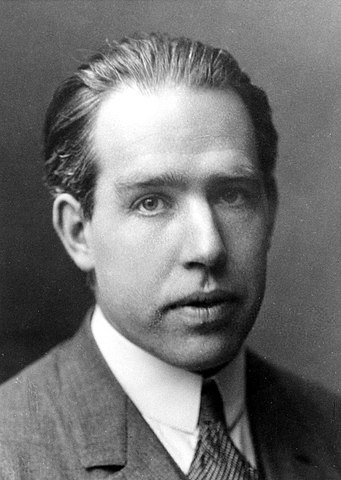
\includegraphics[width=3cm]{../../images/Bohr.jpg}
        \end{column}
        \begin{column}{0.5\textwidth}
            The Bohr Model - Bohr proposed that an atom was a nucleus with electrons "orbiting" in different 
            \pause \alert{energy levels}.
            \vspace{1cm}
        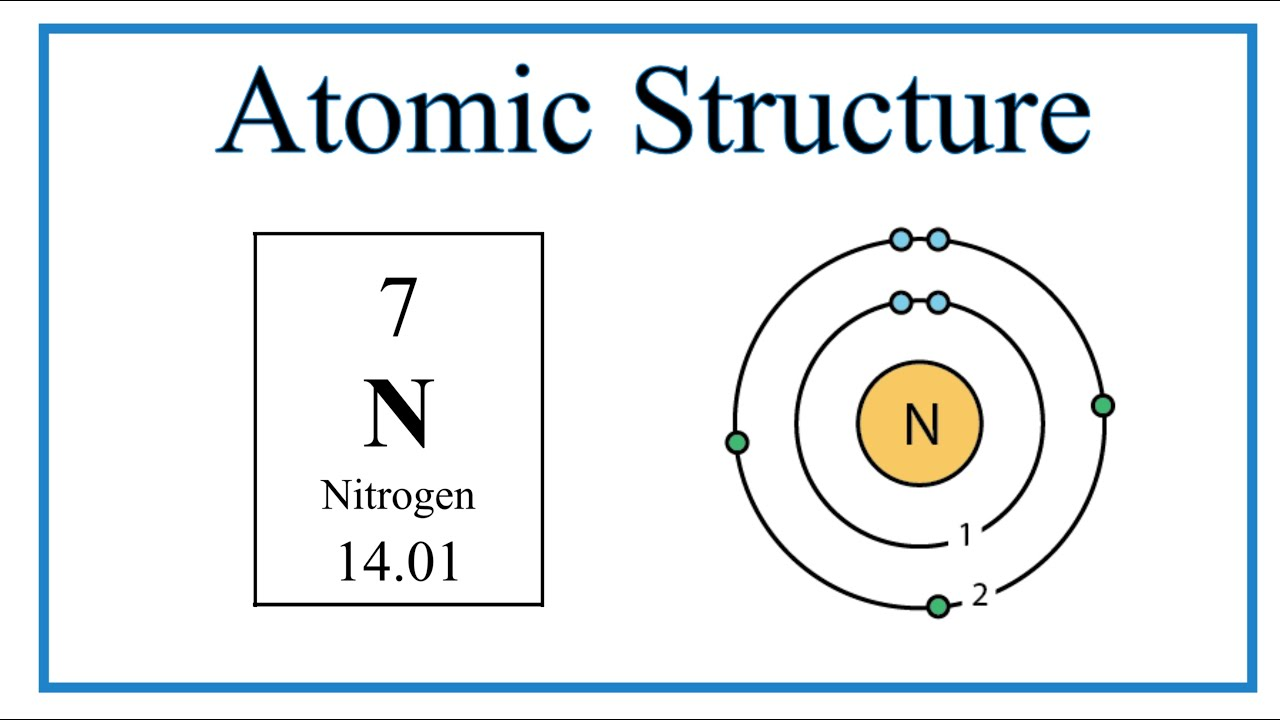
\includegraphics[width=4cm]{../../images/bohr_atom_N.jpg}
        \end{column}
    \end{columns}
\end{frame}

\begin{frame}
    \frametitle{Energy Levels}
    \onslide The electrons closest to the nucleus have the 
    \pause \alert{lowest} 
    \onslide energy, while those further from away have 
    \pause\alert{higher} 
    \onslide energy.
\end{frame}


\end{document}